% !TEX options=--shell-escape
\documentclass[a4paper, 11pt]{article}
\usepackage[utf8]{inputenc}
\usepackage[left=1in,right=1in,bottom=0.8in]{geometry}
\usepackage{enumitem}
\usepackage{graphicx}
\graphicspath{ {Figures/} }
\usepackage{float}
\usepackage[labelfont=bf]{caption}
\usepackage{fixltx2e}
\usepackage{caption}
\usepackage{amsmath}
\usepackage{capt-of}
\usepackage{minted}
\usepackage{tabu}
\usepackage{pgf}
\usepackage{tikz}
\usetikzlibrary{arrows,automata}

\let\svthefootnote\thefootnote


\title{\bf Experiment 3\\\vspace*{2mm} String Recognizer}
\author{\it Amit Kumar | 16D070034}
\date{March 18, 2018}

\begin{document}
\maketitle
\section*{Overview}
In this experiment, we have implemented a \emph{string recognizer} (A sequential circuit using mealy FSM) that can identify the occurrence of the following words.
\begin{itemize}

	\item bomb
	\item gun
	\item knife
	\item terror
	
\end{itemize}

The VHDL code was compiled on Quartus Prime, and simulated using ModelSim which
 % GHDL was also used for simulation purposes, at a low level. This 
 was then uploaded to the {\em Krypton v1.1} 5M1270ZT144C5N CPLD-based board via svf file and urjtag.

% The codes and setup have been covered in section 1. We build the string recognizer piece-wise, by implementing each module independently. The VHDL codes have been kept modular and as generic as possible, for reusability and code clarity. Section 2 presents the simulation observations and miscellaneous results. Section 3 presents the observations after running the scan-chain test on the board.

\section{Setup}
The english alphabet is represented by 5 bits ($\lceil log_2(26) \rceil$), and a bit each for \emph{clock} and \emph{reset} results in 7 input bits which were encoded by converting alphabet position (1-26) to 5-bit binary, for simplicity. I have implemented recognizer for each string individually using FSM mealy model then combined all entities to detect the presence of all four strings .

\subsection{GUN Recognizer}

\begin{figure}[H]
\centering

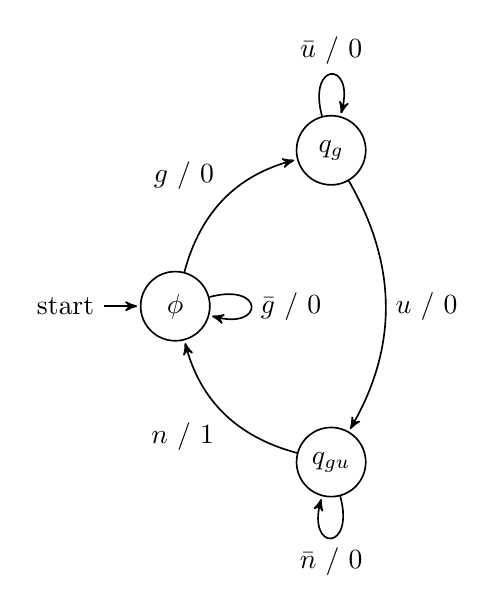
\begin{tikzpicture}[->,>=stealth',shorten >=1pt,auto,node distance=2.8cm,
                    semithick]
  \tikzstyle{every state}=[fill=white,draw=black,text=black]

  \node[initial,state] (A)                    {$\phi$};
  \node[state]         (B) [above right of=A] {$q_g$};
  \node[state]         (D) [below right of=A] {$q_{gu}$};
%   \node[state]         (E) [below of=D]       {$q_e$};

  \path (A) edge        [bend left]      node {$g$ / 0} (B)
        edge [loop right] node {$\bar{g}$ / 0} (A)
        (B) edge [loop above] node {$\bar{u}$ / 0} (B)
            edge    [bend left]          node {$u$ / 0} (D)
%        (C) edge        [bend left]      node {$m$ / 0} (D)
%         edge [loop right] node {$\bar{m}$ / 0} (C)
%             edge [bend left]  node {1,0,R} (E)
        (D) edge [loop below] node {$\bar{n}$ / 0} (D)
            edge [bend left]          node {$n$ / 1} (A);
%         (E) edge [bend left]  node {1,0,R} (A);
\end{tikzpicture}
\caption{Automata Representation for \emph{GUN}}
\end{figure}
Using the above state representation, the encoding has been done as shown below.
\begin{center}
\begin{tabular}{| c | c | c |}
\hline
\bf State & \bf $q_1$ & \bf $q_2$\\
\hline
$\phi$ & 0 & 0 \\
$g$ & 0 & 1 \\
$gu$ & 1 & 0 \\
\hline
\end{tabular}
\end{center}
Following the above state encoding and FSM design (Figure ), the code for detecting \texttt{gun} is given below.
\inputminted[linenos]{vhdl}{GUN.vhd}

\subsection{Bomb Fecognizer}
FSM transition diagram is shown below:
\begin{figure}[h]
\centering

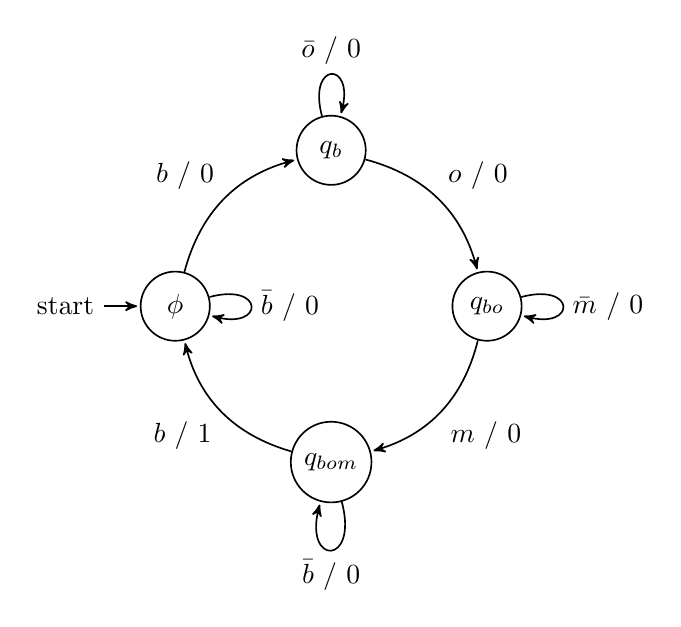
\begin{tikzpicture}[->,>=stealth',shorten >=1pt,auto,node distance=2.8cm,
                    semithick]
  \tikzstyle{every state}=[fill=white,draw=black,text=black]

  \node[initial,state] (A)                    {$\phi$};
  \node[state]         (B) [above right of=A] {$q_b$};
  \node[state]         (D) [below right of=A] {$q_{bom}$};
  \node[state]         (C) [below right of=B] {$q_{bo}$};
%   \node[state]         (E) [below of=D]       {$q_e$};

  \path (A) edge        [bend left]      node {$b$ / 0} (B)
  			edge [loop right] node {$\bar{b}$ / 0} (A)
%             edge              node {1,1,R} (C)
        (B) edge [loop above] node {$\bar{o}$ / 0} (B)
            edge    [bend left]          node {$o$ / 0} (C)
        (C) edge        [bend left]      node {$m$ / 0} (D)
        	edge [loop right] node {$\bar{m}$ / 0} (C)
%             edge [bend left]  node {1,0,R} (E)
        (D) edge [loop below] node {$\bar{b}$ / 0} (D)
            edge [bend left]          node {$b$ / 1} (A);
%         (E) edge [bend left]  node {1,0,R} (A);
\end{tikzpicture}
\caption{Automata Representation for \emph{BOMB }}
\end{figure} \\

As a notation in the above figure, the text on each edge of the graph $a / b$ represents input $a$ to the machine, and output $b$ of the machine.
 % State encoding can be done in a smart way to reduce the combinational overhead for each state bit. For this purpose, I have used \emph{Gray Codes} to encode the states.
\begin{center}
\begin{tabular}{| c | c | c |}
\hline
\bf State & \bf $q_1$ & \bf $q_2$\\
\hline
$\phi$ & 0 & 0 \\
$b$ & 0 & 1 \\
$bo$ &1 & 0 \\
$bom$ & 1 & 1\\
\hline
\end{tabular}
\end{center}
Following the above state assignment and FSM design (Figure 1), the code for detecting \texttt{bomb} is given below.

\inputminted[linenos]{vhdl}{BOMB.vhd}



\subsection{Knife Recognizer}

\begin{figure}[H]
\centering

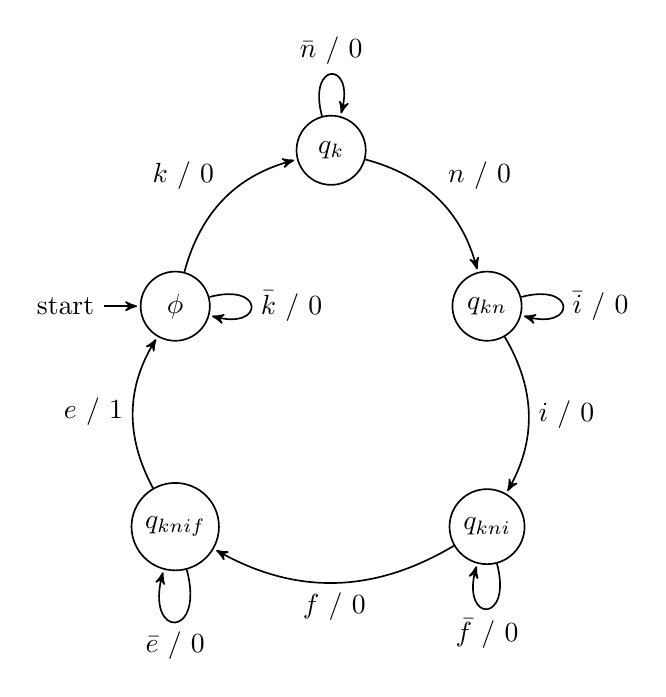
\begin{tikzpicture}[->,>=stealth',shorten >=1pt,auto,node distance=2.8cm,
                    semithick]
  \tikzstyle{every state}=[fill=white,draw=black,text=black]

  \node[initial,state] (A)                    {$\phi$};
  \node[state]         (B) [above right of=A] {$q_k$};
  \node[state]         (D) [below  of=A] {$q_{knif}$};
  \node[state]         (C) [below right of=B] {$q_{kn}$};
   \node[state]         (E) [below of=C]       {$q_{kni}$};

  \path (A) edge        [bend left]      node {$k$ / 0} (B)
  			edge [loop right] node {$\bar{k}$ / 0} (A)
%             edge              node {1,1,R} (C)
        (B) edge [loop above] node {$\bar{n}$ / 0} (B)
            edge    [bend left]          node {$n$ / 0} (C)
        (C) edge        [bend left]      node {$i$ / 0} (E)
        	edge [loop right] node {$\bar{i}$ / 0} (C)
%             edge [bend left]  node {1,0,R} (E)
        (D) edge [loop below] node {$\bar{e}$ / 0} (D)
            edge [bend left]          node {$e$ / 1} (A)
         (E) edge [bend left]  node {$f$ / 0} (D)
         	edge [loop below] node {$\bar{f}$ / 0} (E);
\end{tikzpicture}
\caption{Automata Representation for \emph{KNIFE}}
\end{figure}

Going with the above state representation, the encoding requires 3 bits (5 states), and hence I have shown encoding below.

\begin{center}
\begin{tabular}{| c | c | c | c |}
\hline
\bf State & \bf $q_1$ & \bf $q_2$ & \bf $q_3$\\
\hline
$\phi$ & 0 & 0 & 0 \\
$k$ & 0 & 0 & 1 \\
$kn$  & 0 &1 & 0 \\
$kni$ & 0 & 1 & 1\\
$knif$ & 1 & 0 & 0 \\
\hline
\end{tabular}
\end{center}
Following the above state assignment and FSM design (Figure 3), the code for detecting \texttt{knife} is given below.
\inputminted[linenos]{vhdl}{KNIFE.vhd}

\subsection{Terror Recognizer}

\begin{figure}[H]
\centering

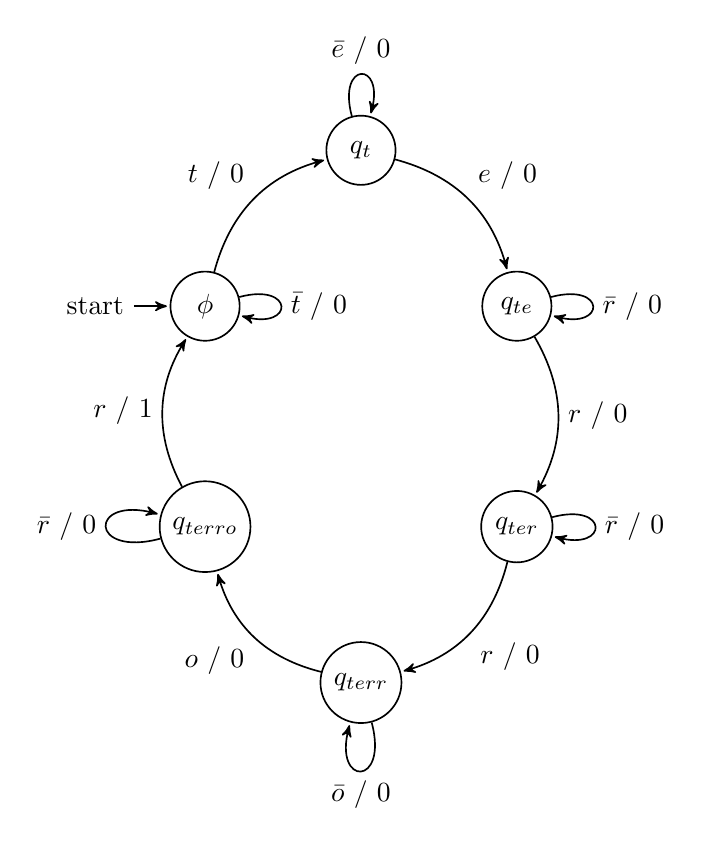
\begin{tikzpicture}[->,>=stealth',shorten >=1pt,auto,node distance=2.8cm,
                    semithick]
  \tikzstyle{every state}=[fill=white,draw=black,text=black]

  \node[initial,state] (A)                    {$\phi$};
  \node[state]         (B) [above right of=A] {$q_t$};
  \node[state]         (D) [below  of=A] {$q_{terro}$};
  \node[state]         (C) [below right of=B] {$q_{te}$};
   \node[state]         (E) [below of=C]       {$q_{ter}$};
   \node [state]			(F) [below left of=E] {$q_{terr}$};

  \path (A) edge        [bend left]      node {$t$ / 0} (B)
  			edge [loop right] node {$\bar{t}$ / 0} (A)
%             edge              node {1,1,R} (C)
        (B) edge [loop above] node {$\bar{e}$ / 0} (B)
            edge    [bend left]          node {$e$ / 0} (C)
        (C) edge        [bend left]      node {$r$ / 0} (E)
        	edge [loop right] node {$\bar{r}$ / 0} (C)
%             edge [bend left]  node {1,0,R} (E)
        (D) edge [loop left] node {$\bar{r}$ / 0} (D)
            edge [bend left]          node {$r$ / 1} (A)
        (F) edge [bend left] node {$o$ / 0} (D)
	        edge [loop below] node {$\bar{o}$ / 0} (F)
         (E) edge [bend left]  node {$r$ / 0} (F)
         	edge [loop right] node {$\bar{r}$ / 0} (E);
\end{tikzpicture}
\caption{Automata Representation for \emph{TERROR}}
\end{figure}
Going with the above state representation, the encoding requires 3 bits (6 states), and hence I used following for encoding the states.
\begin{center}
\begin{tabular}{| c | c | c | c |}
\hline
\bf State & \bf $q_1$ & \bf $q_2$ & \bf $q_3$\\
\hline
$\phi$ & 0 & 0 & 0 \\
$t$ & 0 & 0 & 1 \\
$te$  & 0 &1 & 0 \\
$ter$ & 0 & 1 & 1\\
$terr$ & 1 & 0 & 0 \\
$terro$ & 1 & 0 & 1 \\
\hline
\end{tabular}
\end{center}

Following the above state assignment and FSM design (Figure 4), the code for detecting \texttt{terror} is given below.
\inputminted[linenos]{vhdl}{TERROR.vhd}

\subsection*{Final String Recognizer}
% Now that we have 4 independent FSMs that seem to be doing their job right, we must put them all together, in order to obtain the machine as required in the problem description. Without much effort, this can be done by simply taking an OR operation of the 4 individual outputs. This has been done in the \texttt{DUT}.

Since I have implemented four individual FSMs , following I have combined all four to output '1' if any of the four strings are found . 
\inputminted[linenos]{vhdl}{string_recognizer.vhd}

To map our string recognizer to the input string of tracefile , I have made a final DUT to be used for testbench.
\inputminted[linenos]{vhdl}{DUT.vhd}



\section{Observations}
After implementing the design in code, the next major part is to simulate and test the code for a set of inputs. RTL and Gate-Level simulation was performed on the machine, as a whole. Snapshots of the same are given in Figures 5-8. The validity of the code can be ascertained by the fact that all test cases passed successfully.

For simulation, I have modified the generic testbench given below:
\inputminted[linenos]{vhdl}{Testbench.vhd}
\begin{figure}[H]
\centering
\includegraphics[scale=0.33]{rtl1.png}
\caption{RTL Simulation of the String Detector for tracefile1.txt given }
\end{figure}

\begin{figure}[H]
\centering
\includegraphics[width=10cm]{r1.png}
\caption{RTL Simulation of the String Detector for tracefile1.txt Zoomed-in }
\end{figure}

\begin{figure}[H]
\centering
\includegraphics[scale=0.33]{rtl2.png}
\caption{RTL Simulation of the String Detector for tracefile2.txt given }
\end{figure}

\begin{figure}[H]
\centering
\includegraphics[scale=0.33]{gatelev1.png}
\caption{Gate level Simulation of the String Detector for tracefile1.txt given }
\end{figure}

\begin{figure}[H]
\centering
\includegraphics[width=12cm]{g1.png}
\caption{Gate level Simulation of the String Detector for tracefile1.txt Zoomed-in transcript}
\end{figure} 

\begin{figure}[H]
\centering
\includegraphics[scale=0.33]{gatelevel2.png}
\caption{Gate level Simulation of the String Detector for second tracefile2.txt given }
\end{figure}

\begin{figure}[H]
\centering
\includegraphics[width=12cm]{g2.png}
\caption{Gate level Simulation of the String Detector for second tracefile2.txt Zoomed-in transcript}
\end{figure} 

\begin{figure}[H]
\centering
\includegraphics[width=12cm]{initial_error.png}
\caption{Initial error in Gate level Simulation of the String Detector for second tracefile2.txt Zoomed-in transcript}
\end{figure}


\section{Scan-Chain Tests}

We have tested the logic using the RTL simulations, emulated the CPLD performance using the gate-level simulation and burned svf file of code on the Krypton board using urjtag . Next, we need to check that the code is actually running as it is expected to, on the board. 
Hence, we test the uploaded code on the hardware using the scan-chain setup, as suggested in the manual using scanchain files and Tiva-C microcontroller. This setup was run on a set of two collections of text which has occurrences of the concerned string.

\subsection*{Results}
\begin{figure}[H]
\centering
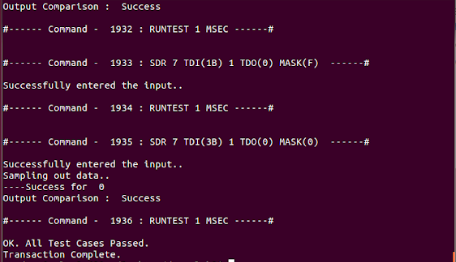
\includegraphics[scale=0.66]{scan_chain.png}
\caption{Screenshot of success of the scan-chain test}
\end{figure}

Since, all the cases passed successfully at all stages and hence the complete string recognizer can be used in hardware, as required.
\end{document}